\documentclass[ENG,PhD]{cinvestav}

%%%%%%%%% PACKAGES
\usepackage[utf8]{inputenc}
\usepackage{color}
\usepackage{latexsym, amssymb}
\usepackage{xcolor}
\usepackage{pstricks}
\usepackage{epsfig}
\usepackage{ucs}
\usepackage{lettrine}
\usepackage{graphicx}
\usepackage{epstopdf}
\usepackage{url}
\usepackage{pseudocode}
\usepackage{ltablex}
\usepackage{rotating}
\usepackage{cite}
\usepackage{csquotes}
\usepackage{lmodern}
\RequirePackage{fix-cm}
\RequirePackage{hyperref}
%\RequirePackage{algorithm}
%\usepackage{algorithmic}
\usepackage{fancybox}
\usepackage{pdflscape} 
\usepackage{multirow}
\usepackage{textcomp}
\usepackage{booktabs}
\usepackage{array}
\newcolumntype{L}[1]{>{\raggedright\let\newline\\\arraybackslash\hspace{0pt}}m{#1}}
\newcolumntype{C}[1]{>{\centering\let\newline\\\arraybackslash\hspace{0pt}}m{#1}}
\newcolumntype{R}[1]{>{\raggedleft\let\newline\\\arraybackslash\hspace{0pt}}m{#1}}
\usepackage{subcaption}

\usepackage[inline]{enumitem}
\newlist{listahorizontal}{enumerate*}{1}
\setlist[listahorizontal]{label=(\alph*)}

\usepackage[ruled]{algorithm2e}
\SetKwComment{tcc}{}{}%

\newcommand{\V}[1]{\mathbf{#1}}

\graphicspath{ {../../../resources/images/} }

\title{Smart Usage of Context Information for the Analysis, Design, and Generation of Power-Aware Policies for Mobile Sensing Apps}
\shorttitle{Smart Usage of Context Information for the Generation of Power-Aware Policies}
\author{Rafael Pérez Torres, César Torres Huitzil and Hiram Galeana Zapién}
\adscripcion{Cinvestav Tamaulipas. Parque Científico y Tecnológico TecnoTam -- Km. 5.5 Carretera Cd. Victoria-Soto La Marina. C.P. 87130 Cd. Victoria, Tamps. }
\city {Cd. Victoria, Tamaulipas, Mexico.}
%\date{December, 2010}
\techreportnumber{0}
\publishedmonth{December} %mes de la publicación
\publishedday{12th} %día de la publicación
\publishedyear{2016} %año de la publicación
\keywords{mobile sensing apps, energy consumption, context information, policy, smartphone}
\correspondingauthor{Rafael Pérez Torres $<$rperez@tamps.cinvestav.mx$>$, César Torres Huitzil $<$ctorres@tamps.cinvestav.mx$>$ and Hiram Galeana Zapién $<$hgaleana@tamps.cinvestav.mx$>$}
\grants{}
\dateofsubmission{December 12th, 2016}
\tobecited{Rafael Pérez Torres, César Torres Huitzil, Hiram Galeana Zapién. Smart Usage of Context Information for the Analysis, Design, and Generation of Power-Aware Policies for Mobile Sensing Apps. CINVESTAV Tamaulipas. 2014 Nov. 31 pp. (No Technical Report No. assigned)}
\placeanddateofpublication{Ciudad Victoria, Tamaulipas, MEXICO.}

\abstract{
This technical report describes the progress and advances developed for the thesis work titled \emph{Smart Usage of Context Information for the Analysis, Design, and Generation of Power-Aware Policies for Mobile Sensing Apps} during the second year of the doctoral program.

In summary, the different efforts during the second year have been focused on producing a solid methodology, powered up by Cognitive Dynamic Systems and Event-Driven Systems concepts, for solving the problems pursued by this research.
A set of experiments have been also performed, validating core aspects of the proposed solution.
}

\begin{document}
\makeintropages

\renewcommand{\baselinestretch}{1.2}

%                                                                                              
%     o             o                          8                       o     o                  
%     8             8                          8                       8                        
%     8   odYo.    o8P   oPYo.   .oPYo.   .oPYo8   o    o   .oPYo.    o8P   o8   .oPYo.   odYo. 
%     8   8' `8     8    8  `'   8    8   8    8   8    8   8    '     8     8   8    8   8' `8 
%     8   8   8     8    8       8    8   8    8   8    8   8    .     8     8   8    8   8   8 
%     8   8   8     8    8       `YooP'   `YooP'   `YooP'   `YooP'     8     8   `YooP'   8   8 
% ::::..::..::..::::..:::..:::::::.....::::.....::::.....::::.....:::::..::::..:::.....:::..::..
% ::::::::::::::::::::::::::::::::::::::::::::::::::::::::::::::::::::::::::::::::::::::::::::::
% ::::::::::::::::::::::::::::::::::::::::::::::::::::::::::::::::::::::::::::::::::::::::::::::
\section{Introduction}
This document presents the summary of advances performed during the last year work in relation to the thesis work entitled: \emph{Smart usage of context information for the analysis, design, and generation of power-aware policies for mobile sensing apps}.

%As an attempt to provide a self-contained document and to ease the comprehension of its content, the research fundamental aspects of the work are also provided.
%More specifically, the rest of this Technical Report is structured as follows.
This Technical Report is structured as follows.
Section~\ref{sec:research-fundamentals} describes the research fundamentals, covering aspects like problem statement, hypothesis, objectives, and contributions.
Section~\ref{sec:theoretical-framework} provides the theoretical framework, including core conceptual elements employed in this research.
Next, Section~\ref{sec:solution} provides a comprehensive description of the solution proposed for addressing the research problem.
The experimental results are presented in Section~\ref{sec:experimental-results}, while future work is described in Section~\ref{sec:future-work}.
Finally, conclusions of this report are provided in Section~\ref{sec:conclusions}.





%                                                                                                                                                                                
%      .oPYo.                                                        8             d'b                         8                                         o             8          
%      8   `8                                                        8             8                           8                                         8             8          
%     o8YooP'   .oPYo.   .oPYo.   .oPYo.   .oPYo.   oPYo.   .oPYo.   8oPYo.       o8P    o    o   odYo.   .oPYo8   .oPYo.   ooYoYo.   .oPYo.   odYo.    o8P   .oPYo.   8   .oPYo. 
%      8   `b   8oooo8   Yb..     8oooo8   .oooo8   8  `'   8    '   8    8        8     8    8   8' `8   8    8   .oooo8   8' 8  8   8oooo8   8' `8     8    .oooo8   8   Yb..   
%      8    8   8.         'Yb.   8.       8    8   8       8    .   8    8        8     8    8   8   8   8    8   8    8   8  8  8   8.       8   8     8    8    8   8     'Yb. 
%      8    8   `Yooo'   `YooP'   `Yooo'   `YooP8   8       `YooP'   8    8        8     `YooP'   8   8   `YooP'   `YooP8   8  8  8   `Yooo'   8   8     8    `YooP8   8   `YooP' 
% :::::..:::..:::.....::::.....::::.....::::.....:::..:::::::.....:::..:::..:::::::..:::::.....:::..::..:::.....::::.....:::..:..:..:::.....:::..::..::::..::::.....:::..:::.....:
% ::::::::::::::::::::::::::::::::::::::::::::::::::::::::::::::::::::::::::::::::::::::::::::::::::::::::::::::::::::::::::::::::::::::::::::::::::::::::::::::::::::::::::::::::
% ::::::::::::::::::::::::::::::::::::::::::::::::::::::::::::::::::::::::::::::::::::::::::::::::::::::::::::::::::::::::::::::::::::::::::::::::::::::::::::::::::::::::::::::::
\section{Research fundamentals}
\label{sec:research-fundamentals} 
As an attempt to provide a self-contained document and to ease the comprehension of its content, the research fundamental aspects of the work are also provided.

\subsection{Motivation}
% from sensors
Technological advances on the computation, sensing and communication dimensions of smartphone devices have contributed to their acceptance by users all around the world~\cite{Campbell2012}.
In particular, the smartphone's sensing dimension is supported by a diversity of sensors that enables the unobtrusive acquisition of context information (e.g., location, user activity, ambient context variables, etc.) from raw sensory data~\cite{Lane2010}.
Such context information represents a highly relevant input for building personalized application services to enhance user experience, for instance, by adapting smartphone's operation autonomously without requiring his or her intervention at all.
Nevertheless, long-term \emph{context-aware applications} must query sensors on a continuous basis, which could significantly impact on energy resources of smartphones~\cite{Macias2013}.
This is because the battery capacity remains as the main challenge of mobile platforms, growing only 5 to 10\% per year~\cite{Ma2012,Evarts2015}, or roughly doubling each 10 years~\cite{Tom2015}.
Even worse, such growth rate is out of pace with respect to energy demands imposed by hardware components and the ever-increasing computing power offered by each new generation of mobile devices~\cite{Yurur2015}.

% from survey and tr-seminar-2
At the same time, it is important to note that since their initial conception, mobile platforms described a layered architecture with a clear focus on managing the heavy interaction with user.
As a result, the support for background running processes and for exploiting the power management capabilities of hardware was discarded, leaving out the power-efficiency of the sensing dimension~\cite{Priyantha2011}.
As a consequence, efficient implementations of power-aware mechanisms that do not jeopardize the accuracy requirements of mobile sensing applications still remain an open challenge, which is augmented by the computational and power constraints of mobile devices, and the long-term and near real-time requirements of these applications.

The GPS receiver is, besides the screen display, one of the most energy hungry components of a smartphone and it is the core component of most of Location-Based Services (LBS) applications~\cite{Perez-Torres2016} (although other mechanisms could be employed by services without a high accuracy requirement, like cellular cell tower and wireless networks location providers).
Thus, the core logic of LBS completely depend on the location-awareness of the mobile device for adapting its behavior according to location changes.
Therefore, it becomes a crucial aspect for these systems to conduct a proper management of GPS receiver towards achieving a reasonable use of the energy resources, which is limited on mobile platforms.
However, reducing the sampling frequency poses an additional challenge, known as the \emph{energy consumption} vs. \emph{accuracy} tradeoff, on which an attempt for reducing energy usage leads to a degradation of the accuracy of location tracking performed from collected data.

The research work reported on this document aims to reduce the energy consumption of LBS inspired by the insight of Cognitive Dynamic Systems (CDS)~\cite{Haykin2006}.
On these systems, which are described later on, there is a memory component that aids the decision making process (in our case, the adaptation of sensors operation) by involving information learned from the environment over short and long windows of time.
Thus, the memory acts as a relevant factor that could break the \emph{energy consumption} vs. \emph{accuracy} tradeoff, allowing to reduce energy consumption without necessarily affecting the accuracy.
% The characteristics of the presented research are described in the following sections.


\subsection{Problem statement}
\label{sub:problem-statement}
Conceptually, the final goal of this research is to design a location provider aware of the energy limitations of the mobile device.
Nonetheless, as the location is a reflection of the mobility patterns described by people, a set of more specific problems that could be addressed are:
\begin{itemize}
  \item First, the identification of the user mobility pattern from sensors data, and
  \item Second, the usage of such mobility information for adapting the sensory operations.
\end{itemize}

Both problems are revised in following sections.

\subsubsection{Problem 1: Identification of mobility patterns}
\label{sub:problem-statement-problem-one}
This research work considers two main types of mobility patterns, according to the level of motion granularity that user can describe.
\begin{itemize}
  \item \textbf{Fine-grain mobility patterns}: They refer to motion related to human activity, for instance, walking and running.
  Fine-grain mobility information refers to movement detected by the device, where the device itself is the frame of reference.
  The accelerometer sensor acts as this reference frame, where positive or negative changes in acceleration are observed by the mobile device.

  In particular, this research considers the fine-grain mobility patterns in the set Patterns  $ = \{ \text{static, walking, running, vehicle} \}$, as they represent a hint for inferring current user speed without involving as much energy consumption as the GPS receiver~\cite{Abdesslem2009}.
  Quantitatively, these patterns could be defined according to typical speeds described by user when moving:
  \begin{itemize}
    \item \textbf{Static}: [0 - 1] m/s.
    \item \textbf{Walking}: (1 - 2] m/s.
    \item \textbf{Running}: (2 - 3] m/s. %\{3m/s = 10.8 km/hr, or 5.55 min/km\}
    \item \textbf{Vehicle}: (3 - more) m/s.
  \end{itemize}

  \item \textbf{Coarse-grain mobility patterns}: They refer to motion at large scale (place level), related to distance traversed by user.
  Coarse-grain mobility information can be detected by the mobile device in accordance with an absolute, and external, frame of reference.
  The GPS receiver can detect the global position of the device by means of location coordinates composed by latitude, longitude, and altitude values.
  Nevertheless, a coarse-grain mobility pattern with a higher level of semantic meaning is the idea of a stay point and the arrival and departure of user to and from them, respectively.
  The stay points, formally described in following sections, are derived from the stream of location updates and represent places the user holds an interest with.

  Qualitatively, the detection of arrival and departure events of a stay point provides relevant information for reducing the access to GPS receiver, as it could be disabled when user is inside a stay point.
\end{itemize}

Having defined the previous elements, the problem of identification of mobility patterns is stated as follows:
\begin{displayquote}
Given a set of values $\mathcal{V} = v_1,v_2,\ldots,v_n$ obtained from sensor $\mathcal{S}$ in time range $[t_1,t_2]$, identify coarse-grain or fine-grain mobility information:
$$
\text{PatternIdentifier}(\mathcal{V}) \rightarrow p_S \in \text{Patterns}
$$
where Patterns  $ = \{ \text{static, walking, running, vehicle} \}$ for fine-grain location information, while for coarse-grain information refers to the arrival and departure to-from stay points described by user's mobility.
Additionally, the sensor $\mathcal{S}$ for fine-grain information is \verb|accelerometer|, while sensor $\mathcal{S}$ for coarse-grain information is \verb|GPS|.
\end{displayquote}

\subsubsection{Problem 2: Generation of policies for adapting sensory operations}
\label{sub:problem-statement-problem-two}
The second problem addresses how to use the detected mobility information towards adapting sensory operations while considering an accuracy requirement and the current status of smartphone constraints (i.e., the battery level).
Formally, this problem is stated as follows:

\begin{displayquote}
Given a set of detected mobility patterns $\mathcal{P} = \{ p_{S_1}, p_{S_2}, \ldots, p_{S_n} \}$ in historical sensors data, accuracy requirements of mobile app $a$, and physical constraints status $c$ of the mobile device, design a policy that selects the proper set of sensors $\mathcal{S}_{new}$ and its associated configuration $\mathcal{S}_{new_{conf}}$  while meeting application requirements and reducing energy consumption.
$$
  \text{PolicyGeneration}( \mathcal{P}, a, c ) \longrightarrow{} \mathcal{S}_{\text{new}}, \mathcal{S}_{\text{new}_{\text{conf}}}
$$

The $\mathcal{S}_{\text{new}_{\text{conf}}}$ configuration is referred as the \emph{adaptive duty cycle} of associated sensor.
\end{displayquote}


\subsection{Hypothesis}
In order to tackle the aforementioned problems, this research work proposes the following hypothesis:
\begin{displayquote}
  Dynamic policies driven by events detected in user mobility could reduce energy consumption of the mobile device when performing continuous location tracking.
  User mobility could be expressed by means of a spatial-time model learned from short and long time windows of context information extracted from GPS and accelerometer sensors data.
\end{displayquote}

By dissecting such hypothesis, it could be found a link with the previous problem statements, since there is a task for detecting \textbf{mobility events}, and other task referring to the usage of \textbf{dynamic policies}.
We assume that a dynamic policy is a special rule that defines how sensors should be accessed in order to reduce the energy consumption and achieve mobile app requirements. 
The context information from where policies are built, refers to the information obtained by analyzing data coming from sensors.
Also, the hypothesis makes reference to a \emph{spatial-time model}, which defines the memory attribute of the proposed solution as the mechanism for breaking the \emph{energy consumption} vs. \emph{accuracy} tradeoff.


\subsection{Objectives}
The main objective of this research work is:
\begin{itemize}
  \item To reduce energy consumption in the mobile sensing apps, which perform continuous sensor readings, through self-adapting power-aware policies generated from context information obtained from sensors data.
\end{itemize}

Similarly, the particular objectives are:
\begin{itemize}
  \item To identify mobility patterns from context information obtained from an inertial sensor (accelerometer) and location providers (GPS).
  \item To generate policies for a self-adapting sensors' usage from identified mobility patterns, accuracy and energy requirements of mobile application, and status of mobile device's constraints.  OR
  \item To generate an accurate representation of mobility patterns, which in conjunction with mobile app accuracy requirements and mobile device constraints, allows to create power-aware GPS sensing policies.
  \item To ease the development of mobile sensing applications that require user location tracking, i.e., LBS, isolating the complexity of sensors' access and the associated efficient energy management.
\end{itemize}


\subsection{Contributions}
The contributions aimed by this research work are:
\begin{itemize}
  \item A mechanism for detecting mobility patterns from the data collected by mobile device's sensors (in particular, GPS and accelerometer).
  \item A mechanism for generating sensors sampling policies, which employs mobile app's requirements (accuracy requirement), status of mobile device constraints (battery level), and user's mobility information (using the pattern detected by previous mechanism).
  The produced policies allow to perform an intelligent usage of smartphone's sensing facilities in continuous sensor sampling tasks, reducing the energy consumption.
  \item A middleware implementing the previous power-aware mechanisms for easing the development of location based services for the Android mobile platform.
\end{itemize}


\subsection{Methodology}
The overall research work pursued in this thesis is divided in the following methodology steps.
\begin{enumerate}
  \item \textbf{Familiarization with state-of-art power-aware sensing related techniques.}
  A review of state-of-art power-aware related techniques has been performed.
  Relevant concepts, alternative insights and future trends have been identified from this state-of-art revision.
  
  \item \textbf{Formal definition and selection of mobility patterns to be identified.}
  After a study of the different mobility attributes described by user, the previously defined fine-grain and coarse-grain mobility patterns have been selected as the user mobility characteristics to be identified and exploited.

  \item \textbf{Research on pattern recognition algorithms focused on mobility patterns identification.}
  From literature, it has been selected a strategy for identified user activity from accelerometer data through a HAR module (Human Activity Recognition).% powered by a Naive Bayes classifier.
  Similarly, an event-driven variant of a trajectory analysis algorithm for stay points detection has been developed and tested.
  Finally, a Geofencing mechanism, which employs the stay points produced by the previous algorithm, has been also proposed and tested for identifying the arrival and departure events to and from such places.
  
  \item \textbf{Design of the Pattern Identification Element (PIE).}
  A global-integrator module has been built for detecting the fine and coarse-grain mobility patterns from sensors data, as well as for supporting the storage of the events arisen from those notifications in a memory component.
  

  \item \textbf{Research on and proposition of adaptive policies for energy efficient usage of sensors.}
  A relevant task for this research is the employment of the learned information for defining power-aware policies for conducting sensor sampling adaptations.
  Intuitively, policies have to reduce sampling frequency of GPS when user is inside a stay point and adapt the sampling frequency when user is moving between stay points according to the speed of the activity described by user.
    

  \item \textbf{Design of the Policy Generation Element (PGE).}
  All of the findings on the policies generated in previous points have to be included in a logic component able to exploit them when user is describing actual motion.
  The module must also consider the mobile app's accuracy requirement and the level of mobile device's constraints (battery level).
  

  \item \textbf{Development of a middleware involving the PIE and PGE for the Android platform.}
  Both modules, PIE and PGE, have to be implemented as a middleware for a mobile platform (in this case Android).
  Although they could be considered as technical tasks, there are several pitfalls for the implementation of such software unit, as the management of different power states of mobile device and other Android aggressive power saving mechanisms have to be addressed or overridden.

  \item \textbf{Experimentation in terms of accuracy and energy efficiency.}
  The experimentation consists on the evaluation of the performance of proposed system solution in terms of energy consumption and location tracking accuracy, both at the spatial and time dimensions.
  This means that distance aspects when user is commuting between stay points, and the arrival and departure time events (to and from) stay points must be measured.
\end{enumerate}





%                                                                                                                                                                             
%     ooooo   8                                             o     o                     8        d'b                                                                    8      
%       8     8                                             8                           8        8                                                                      8      
%       8     8oPYo.   .oPYo.   .oPYo.   oPYo.   .oPYo.    o8P   o8   .oPYo.   .oPYo.   8       o8P    oPYo.   .oPYo.   ooYoYo.   .oPYo.   o   o   o   .oPYo.   oPYo.   8  .o  
%       8     8    8   8oooo8   8    8   8  `'   8oooo8     8     8   8    '   .oooo8   8        8     8  `'   .oooo8   8' 8  8   8oooo8   Y. .P. .P   8    8   8  `'   8oP'   
%       8     8    8   8.       8    8   8       8.         8     8   8    .   8    8   8        8     8       8    8   8  8  8   8.       `b.d'b.d'   8    8   8       8 `b.  
%       8     8    8   `Yooo'   `YooP'   8       `Yooo'     8     8   `YooP'   `YooP8   8        8     8       `YooP8   8  8  8   `Yooo'    `Y' `Y'    `YooP'   8       8  `o. 
% ::::::..::::..:::..:::.....::::.....:::..:::::::.....:::::..::::..:::.....::::.....:::..:::::::..::::..:::::::.....:::..:..:..:::.....:::::..::..:::::.....:::..::::::..::...
% :::::::::::::::::::::::::::::::::::::::::::::::::::::::::::::::::::::::::::::::::::::::::::::::::::::::::::::::::::::::::::::::::::::::::::::::::::::::::::::::::::::::::::::
% :::::::::::::::::::::::::::::::::::::::::::::::::::::::::::::::::::::::::::::::::::::::::::::::::::::::::::::::::::::::::::::::::::::::::::::::::::::::::::::::::::::::::::::
\section{Theoretical framework}
\label{sec:theoretical-framework} 
A rich body of research towards the design of power-aware sensing techniques for mobility smartphone-based sensing systems has been reported in literature~\cite{Perez-Torres2016}.
%There is reported in the literature a rich body of research for designing power-aware sensing techniques for mobility oriented smartphone-based sensing systems~\cite{Perez-Torres2016}.
As such, a power-aware sensing technique is one that adapts the management of sensors while considering the limited energy of the mobile platform.
This sensors management process could be based on received sensory data, which in turn could be analyzed and explored through machine learning techniques for detecting relevant information for adapting sensors operation.
Nonetheless, the proposed system solution distinguishes among existing ones because of its inspiration on CDS and other valuable elements for going beyond a typical machine learning scheme and achieve a power-aware location tracking mechanism.
The benefits of relying on a dynamic system, besides the power savings, also include an increase of the awareness of mobile device about activities performed by user, bringing cognitive attributes to the smartphone~\cite{Campbell2012}.

The fundamental pillars of this research work are described in following sections.

\subsection{Physics' perspective of motion}
One of the fundamental concepts for the research are the points of interest (POI) or \textbf{stay points} which enable the platform to identify the most common places the user visits.
%\subsubsection*{Stay points}
A stay point refers to a geographical zone where the user has been for a considerable amount of time.
Semantically, it describes a part of the world the user holds a special interest with.
Formally, a stay point is a virtual location defined by latitude (\emph{lat}), longitude(\emph{lon}), arrival time (\emph{at}) and departure time (\emph{dt}) components, and is calculated from a set of consecutive GPS fixes $\mathbf{P}=\{p_{m},p_{m+1},\ldots,p_{n}\}$, were each of these fixes is in turn composed by latitude, longitude and timestamp (\emph{t}).

Building a stay point requires a distance $\theta_{d}$ and a time $\theta_{t}$ threshold, and its composition must observe:
\begin{equation}
  \left|p_{n}.T-p_{m}.T\right|\geq\theta_{t}
  \label{eq:poi-constraint-one}
\end{equation}
and
\begin{equation}
  \text{distance}(p_{m},p_{i})\leq\theta_{d}, \forall m<i\leq n
  \label{eq:poi-constraint-two}
\end{equation}

Equation~\ref{eq:poi-constraint-one} controls the amount of time that user should spent inside a stay point, whereas Equation~\ref{eq:poi-constraint-two} constraints the size of the geographical area referenced by the stay point.
The calculation of the centroid \emph{lat} and \emph{lon} features of a $\mathbf{x}$ stay point is performed in terms of a simple arithmetic mean as expressed in Equations~\ref{eq:centroid-latitude} and \ref{eq:centroid-longitude}.
The \emph{at} and \emph{dt} components are obtained from the timestamps of the $p_m$ and $p_n$ fixes, respectively.

\begin{equation}
\mathbf{x}.lat = \frac{ \sum_{i=m}^{n}p_{i}.Lat }{ |\mathbf{P}| }\label{eq:centroid-latitude}
\end{equation}

\begin{equation}
\mathbf{x}.lon = \frac{ \sum_{i=m}^{n}p_{i}.Lngt }{ |\mathbf{P}| }\label{eq:centroid-longitude}
\end{equation}

The stay points then represent anchor points in the mobility of user, and once obtained (including the average arrival and departure times), could represent a highly valuable information for disabling or at least reducing the sampling frequency of GPS when user is inside them.

Similarly, the fine-grain activity information derived from sensors (in this case accelerometer) represents an important hint for inferring the speed described by user when moving between stay points, without causing a high energy consumption as in the case of GPS receiver.

From the speed point of view, stay points represent those intervals on which the speed is near to 0 m/s, while the commuting between stay points is described by such intervals on which speed is greater than 0 m/s. 
As a consequence, increments and decrements on acceleration values could then represent the departures and arrivals from and to stay points, respectively, as depicted in Figure~\ref{fig:physics-perspective-of-motion}.

\begin{figure}
  \centering
  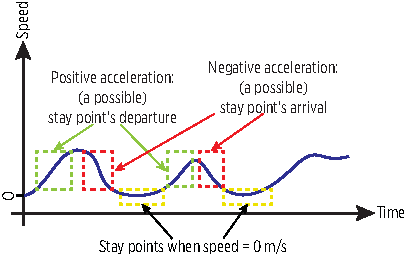
\includegraphics[]{vectors/physics-perspective-of-motion}
  \caption{The physics perspective of motion considered in this research.}
  \label{fig:physics-perspective-of-motion}
\end{figure}

There are different families of algorithms aimed at detecting stay points from a given GPS trajectory~\cite{Lee2013a}, which are briefly described as follows:
\begin{itemize}
  \item \textbf{Clustering-based strategies}: Clustering algorithms are employed for grouping raw coordinates into places.
  These algorithms could only consider spatial distance aspects (as in the DBSCAN algorithm~\cite{Ester1996}) or also involve the time dimension (as in DJ-Cluster~\cite{Zhou2007} and CB-SMoT~\cite{Palma2008}).
  \item \textbf{Differential-based strategies}: Algorithms are based on the analysis of time and spatial differences between individual GPS fixes for finding centroids that represent a stay point (as in~\cite{Kang2005,Hu2007,Li2008,Ye2009}).
  \item \textbf{Probabilistic-based strategies}: Algorithms under this category try to infer the most frequently visited places from location data by using probabilistic models, like Gaussian Mixture Models (as in~\cite{Zhang2007}), Bayesian models (as in~\cite{Nurmi2008}), and Conditional Random fields (as in~\cite{Liao2013}).
\end{itemize}

Because of the low computational complexity and streaming nature for calculating the time and spatial differences between individual GPS fixes, differential-based algorithms are more suitable for conducting stay points detection in smartphones~\cite{Lee2013a}.
However, it is important to note that existing differential-based algorithms are aimed at an off-line analysis of complete GPS trajectories.
Nonetheless, as the source of location updates is an asynchronous stream of GPS fixes, such calculation of differences could be performed right after each location update is received.
Following this guideline, differential-based algorithms could be adapted for observing an event-driven approach.
In particular, the algorithm proposed by Li \emph{et al.}, was adapted for allowing the on-line detection of stay points.
Once a new location fix that fulfils the algorithm's specific conditions is received, a stay point could be generated and notified to subscribed modules.

The steps of Li's algorithm are shown in Algorithm~\ref{alg:generic_event_driven_algorithm}.
The generic aspects of this adapted version relies on Lines~\ref{alg:line-incorporateData} and \ref{alg:line-reset-collected-data}, which define how each incoming event notification (i.e., the location update) is processed, and how the accumulated sub-trajectory data is reset, respectively.
For instance, depending on algorithm design aspects, the Line~\ref{alg:line-incorporateData} could represent the storing of the incoming location updates into an internal buffer, or just simply the accumulation of their coordinate values in the \texttt{collectedData} variable.
%As it will be explained later on in Section~\ref{sec:implementation}, such implementation variants are possible since differential algorithms rely on the centroid concept.
Depending on how the location updates are collected and managed by the algorithm, Line~\ref{alg:line-reset-collected-data} must properly reset the buffer or the accumulated location coordinates and then incorporate the $p_{\texttt{last}}$ location fix.
Finally, the Line~\ref{alg:line-calculate-centroid} is aimed at calculating the centroid's coordinates of the stay point, using Equations~\ref{eq:centroid-latitude} and \ref{eq:centroid-longitude}.


\begin{algorithm}[t]
\small
\DontPrintSemicolon
\LinesNumbered
\SetCommentSty{mycapfn}
\KwData {A stream of GPS location updates $\mathcal{S}$, a distance threshold $\theta_d$, and a minimum time threshold $\theta_{t_{\text{min}}}$}
\KwResult {A stream of calculated stay points $\mathcal{O}$}
% \SetKwFunction{restartSubtrajectory}{resetCollectedData}

\While {Stream $\mathcal{S}$ \emph{is active}}{
    \BlankLine
    Incorporate $\mathcal{S}$.\texttt{incomingUpdate} into \texttt{collectedData} \label{alg:line-incorporateData} \;

    \BlankLine
    \If{ $ \text{\textbf{\emph{distance}}}(p_{\texttt{\emph{first}}},p_{\texttt{\emph{last}}}) >\theta_d$}{
        \BlankLine
        \If{ $ \text{\textbf{\emph{timeDifference}}}(p_{\texttt{\emph{first}}},p_{\texttt{\emph{last}}})>\theta_{t_\text{min}}$}{
            $\pi \leftarrow $ Calculate centroid using \texttt{collectedData} \label{alg:line-calculate-centroid} \;
            Output $\pi$ in $\mathcal{O}$
        }
        \texttt{resetCollectedData($p_{\text{last}}$)} \label{alg:call-restart-subtrajectory} \label{alg:line-reset-collected-data}\;
    }
}
\caption{A generic event-driven adaptation of Li's algorithm for conducting on-line stay points detection\label{alg:generic_event_driven_algorithm}.}
\end{algorithm}

\subsection{Event-driven systems}
Event-driven systems are those systems that rely on information detected from outside (environment) and that react according to changes on such information.
An event is an occurrence within a particular system or domain; it is something that has happened, or is contemplated as having happened in that domain~\cite{Etzion2011}.

The top-level architecture of an event-driven system mainly consists of three logical layers: 
\begin{listahorizontal}
  \item \emph{event sources},
  \item \emph{event processing}, and
  \item \emph{event handling}
\end{listahorizontal}, as shown in Figure~\ref{fig:event-based-system-architecture}, which is focused on the stay points detection process.
The events have to be processed immediately when they occur, requiring a continuous background execution so that a significant situation could be detected promptly.

\begin{figure}
  \centering
  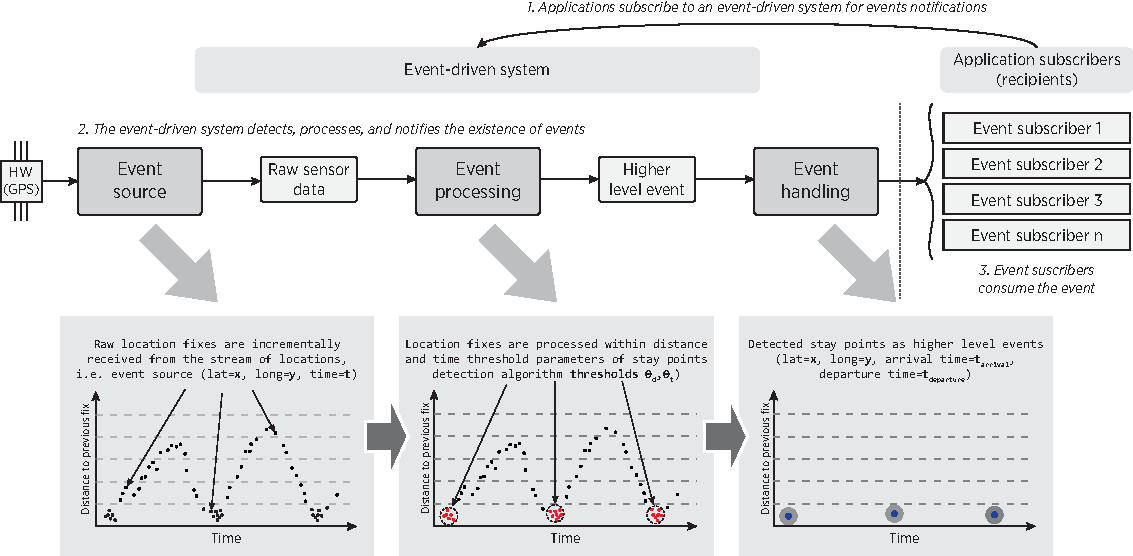
\includegraphics[width=\textwidth]{vectors/event-driven-system}
  \caption{Top-level architecture of an event-driven system.}
  \label{fig:event-based-system-architecture}
\end{figure}

Under the event-oriented viewpoint, an \emph{event source} is a system component that is capable of producing a stream of observations corresponding to events occurring in a given environment.
% As such, the GPS receiver is considered this event source, which is continuously producing a stream of location update events.
The next fundamental component is an \emph{event processing} engine that incrementally processes the stream of incoming events and produces more complex events or actions with a valuable semantic meaning.
%Here, the algorithm for stay points detection is uninterruptedly running in the background, processing the stream of location updates, and serving to concurrent applications, even during the stand-by modus.
Finally, an \emph{event handling} component employs the processed events and reacts accordingly by triggering a specific-domain action.


\subsection{Cognitive Dynamic Systems (CDS)}
CDS represent an integrative field whose study involves fields rooted in neuroscience, cognitive science, computer science, mathematics, physics, engineering, and more~\cite{Haykin2006,Haykin2012}.
A system is considered \emph{dynamic} if \emph{time} plays a key role in its input-output behavior.
In general, CDS are inspired by the neural computation capability of the human brain and the perspective that human cognition is a form of computation.
A dynamic system is said to be \emph{cognitive} only if it performs four fundamental tasks basic to human cognition:
\begin{enumerate}
  \item The \emph{perception-action} cycle, which is aimed at maximizing information gaining about the environment.
  \item Memory, in a multilayer scheme that is organized to predict the consequences of actions
  \item Attention, as a way to prioritize the selection and allocation of resources
  \item Intelligence, as for continuous self-adjustment through an adaptive process for responding to new changes in the environment and to create new forms of action and behavior.
\end{enumerate}

A more detailed description of these tasks is given in the next sections.

\subsubsection*{The perception-action cycle}
The perception-action cycle of a CDS refers to a global feedback cycle that comprehends observing data from the environment, processing such data, and taking a decision for actuating (modifying) the environment.
Figure~\ref{fig:cds-perception-action-cycle} presents the perception-action cycle on its most generic sense.
The perception-action cycle involves:
\begin{itemize}
  \item the global feedback loop for maximizing information gain about the environment;
  \item multiscale memory organized to predict the consequences of actions;
  \item an attentional mechanism that prioritizes the allocation of resources; and
  \item a feedback based decision-making mechanism that identifies intelligent choices in uncertain environments.
\end{itemize}

The individual elements involved in the perception-action cycle are described in following sections.

\begin{figure}
  \centering
  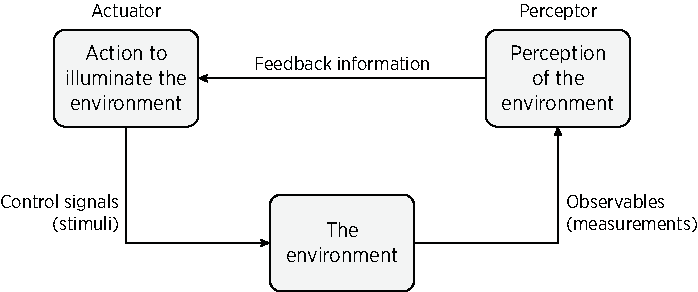
\includegraphics[scale=0.75]{vectors/cds-generic}
  \caption{The perception-action cycle of a CDS in its most generic sense. Adapted from~\cite{Haykin2012}.}
  \label{fig:cds-perception-action-cycle}
\end{figure}

\subsubsection*{Memory}
Memory allows a CDS to maintain a virtual model of the observed environment and its associated information.
The structure of memory is preferably of a multilayer stack, on which each level could represent information at an increasing level of abstraction and/or at different levels of time.
The construction of such model is performed based on the perceptual information and the feedback information obtained from actions performed.
% In CDS, there is a difference between knowledge and memory:
% \begin{itemize}
%   \item \textbf{Knowledge} is a memory of certain facts and relationships that exist between them, none of which changes with time: knowledge is static in its contents.
%   \item \textbf{Memory} is dynamic, its contents continually changes over the cource of time in accordance with changes in the environment.
% \end{itemize}
% In other words, contents of memory are subject to time contraints, whereas knowledge is timeless, free of time constraints.

As a CDS is composed by a perceptor and an actuator, memory can be classified as perceptual and executive memory, respectively.
Thus the memory also acts as a concentrator component that maintains a snapshot of current state of system components, and allows the information feedback with the perceptor and actuator blocks.

\subsubsection*{Perceptual memory}
Perceptual memory refers to the experiential knowledge gained by the perceptor through a process of learning from the environment, such that the contents of the memory continually change with time in accordance to changes in the environment. % --> OUR PIPELINES OR CLASSIFIERS
As a result, perceptual memory defines an internal library with elements that represent items of knowledge about the environment.
% Perceptual memory is also coupled to an evironmental scene analyzer, involving:
% \begin{itemize}
%   \item Retrieval of old memory representing features learned about the environment in past stimuli and
%   \item Updating the old memory according to new information about the environment contained in the incoming stimuli.
% \end{itemize}

\subsubsection*{Executive memory}
Executive memory is the experiential knowledge gained by the actuator through the lessons learned from actions taken in the environment by the actuator itself, with contents of the memory changing with time in accordance with how the perceptor perceives the environment. % -->OUR POLICY MANAGER
The executive memory also has a library with elements that define items of knowledge about possible action in the environment.
% The executive memory is also coupled to an environmental scene actuator, involving:
% \begin{itemize}
%   \item Retrieving old memory learned about decisions made in the past and
%   \item Updating the old memory with new information about the environment obtained in an indirect manner via the feedback link from the perceptor.
% \end{itemize}


The insight of memory is implied in the proposed hypothesis, as the usage of the learned mobility information is a key component for adapting sensory operations, and because there are different time intervals on which memory ought to be structured and processed.

\subsubsection*{Attention}
The purpose of attention is to allocate selectively the available computational resources to execute a goal-directed action.
Attention is a mechanism that protects, both the perceptual-processing power of the perceptor and the decision-making power of the actuator, from the information-overload problem by prioritizing how the computational resources are allocated.

% For the scope of this research, attention is achieved when the operation of sensors (i.e., resources) is adapted according to changes in mobility, with the final goal of performing user location tracking while reducing energy consumption.

\subsubsection*{Intelligence}
Intelligence is the main feature of a CDS and refers to its ability for continually adjusting itself through an adaptive process by making the perceptor respond to new changes in the environment so as to create new forms of action and behavior in the actuator.
This feature is powered by the perception-action cycle, which considers feedback loops distributed throughout the system.
% Such feedback is the facilitator of computational intelligence, as it controls the interactions between the perceptual and executive parts of the system and manifests itself both globally and locally.
The intelligence is then manifested as a decision-making mechanism in the actuator of a CDS, using probabilistic inference to pick intelligent choices in the face of unavoidable uncertainties in the environment.

% For the presented research, the intelligence performs the actual decision for making adaptations in sensory operations, specifically as a \emph{policy generator element}.

% The efficiency of intelligence can be measured as follows.
% \emph{Through the use of an optimal control algorithm in the actuator, a CDS becomes increasingly more intelligent whereby a prescribed cost-to-go function is progressively reduced and with  it, information about the environment is more efficiently utilized from one cycle to the next.}





 
%                                                              
%     .oPYo.            8              o     o                  
%     8                 8              8                        
%     `Yooo.   .oPYo.   8   o    o    o8P   o8   .oPYo.   odYo. 
%         `8   8    8   8   8    8     8     8   8    8   8' `8 
%          8   8    8   8   8    8     8     8   8    8   8   8 
%     `YooP'   `YooP'   8   `YooP'     8     8   `YooP'   8   8 
% :::::.....::::.....:::..:::.....:::::..::::..:::.....:::..::..
% ::::::::::::::::::::::::::::::::::::::::::::::::::::::::::::::
% ::::::::::::::::::::::::::::::::::::::::::::::::::::::::::::::
\section{Proposed solution}\label{sec:solution}
The proposed solution consists on a middleware for mobile platforms, which has been designed upon the pivotal aspects described in Section~\ref{sec:theoretical-framework}.
The solution is inspired on those fundamental aspects as they aid the identification of mobility patterns and their consumption for self-adapting sensory operations, which are aspects deeply related with the problems pursued by this research.

In general terms, performing mobility tracking in a power-aware manner is highly related with the concept of stay points.
Indeed, the first step towards reducing energy consumption when providing mobility tracking services could be represented by the identification and learning of stay points, which are tasks bound to the first problem of this research (described in Section~\ref{sub:problem-statement-problem-one}).

When information about stay points is known, both in time and space dimensions, it could be exploited for reducing GPS sampling frequency when user is inside them.
Similarly, when user is moving between stay points, the activity information could be employed has a hint of user speed for adapting GPS sampling frequency accordingly.
Both tasks are linked to the second problem of this research (described in Section~\ref{sub:problem-statement-problem-two}).

Therefore, the overall solution is aimed at performing the following goals:
\begin{itemize}
  \item Identify and learn the stay points for reducing GPS sampling frequency inside them.
  \item Infer and/or detect the departure and arrival of user from and to such places.
\end{itemize}

For this last point, the inference process means that the departure time could be inferred from historical data (for instance, the average of stay point's leaving times).
On the other hand, the detection process refers to employing actual sensors data for a prompt identification of the event.

As a requirement for these tasks, the system solution has to identify the next mobility modes:
\begin{itemize}
  \item \texttt{onStayPoint} mode: Refers to when user is inside a stay point.
  \item \texttt{onTrajectory} mode: Refers to when user is moving between stay points.
\end{itemize}

When any of these coarse-grain mobility modes are detected, an event notification is generated, which allows the platform to trigger the associated event processing in a CDS.
% The implementation of the proposed solution is deeply related to the achievement of these tasks, as described in the following section.

The description of the solution is divided in two steps.
First, the conceptual components and their interaction is presented.
Secondly, the materialization of the conceptual framework is provided, presenting its cognitive aspects and the low level operations carried on.

\subsection{Overall conceptual description}
Broadly speaking, the components of the proposed solution feature the fundamental pillars described in the theoretical framework (Section~\ref{sec:theoretical-framework}) as follows.
Regarding the physics' perspective of motion, the solution relies on the concept of stay point as an element for aiding the representation of user mobility. 
Besides acting as anchor points in user mobility, the stay points also represent idle coarse-grain mobility intervals on which disabling GPS could potentially achieve high power savings, without jeopardizing the accuracy of location tracking.

In relation to Event-Driven Systems, the operation of the solution is fully event-driven, reacting to specific events generated by changes in user mobility.
Such events refer to those changes in the coarse and fine-grain mobility patterns described in Section~\ref{sec:research-fundamentals}.
The focus on this class of systems arises from their power-aware design, as their components are activated only upon the reception of event notifications~\cite{Rawassizadeh2015,Lee2015,Duffy2007}.
Similarly, as they are based on message notifications, their components could be logically separated and operate agnostic about the details that originated the event, which is an attribute that favors their loose coupling~\cite{Faison2011,Etzion2011}.

Finally, the proposed solution is highly inspired on CDS concepts. 
First, it actuates after perceiving and processing changes in mobility information.
In this regard, sensors data are explored for detecting and learning mobility patterns, and a sampling adaptation is made for tuning the configuration of sensors (i.e., the affectation on the environment).
Such reaction is also assisted by a memory component that allows the system to obtain an accurate representation of user mobility, which is expressed by means of a spatial-time model.
Also, the reaction of the system exposes intelligence, as it adapts dynamically to changes detected over time.
Similarly, the system features attention capabilities for modifying the list of sensors employed for detecting mobility changes, and for focusing on memory information that results meaningful for adapting sensory operations, rather than on irrelevant data.

\begin{landscape}
\begin{figure}
  \centering
  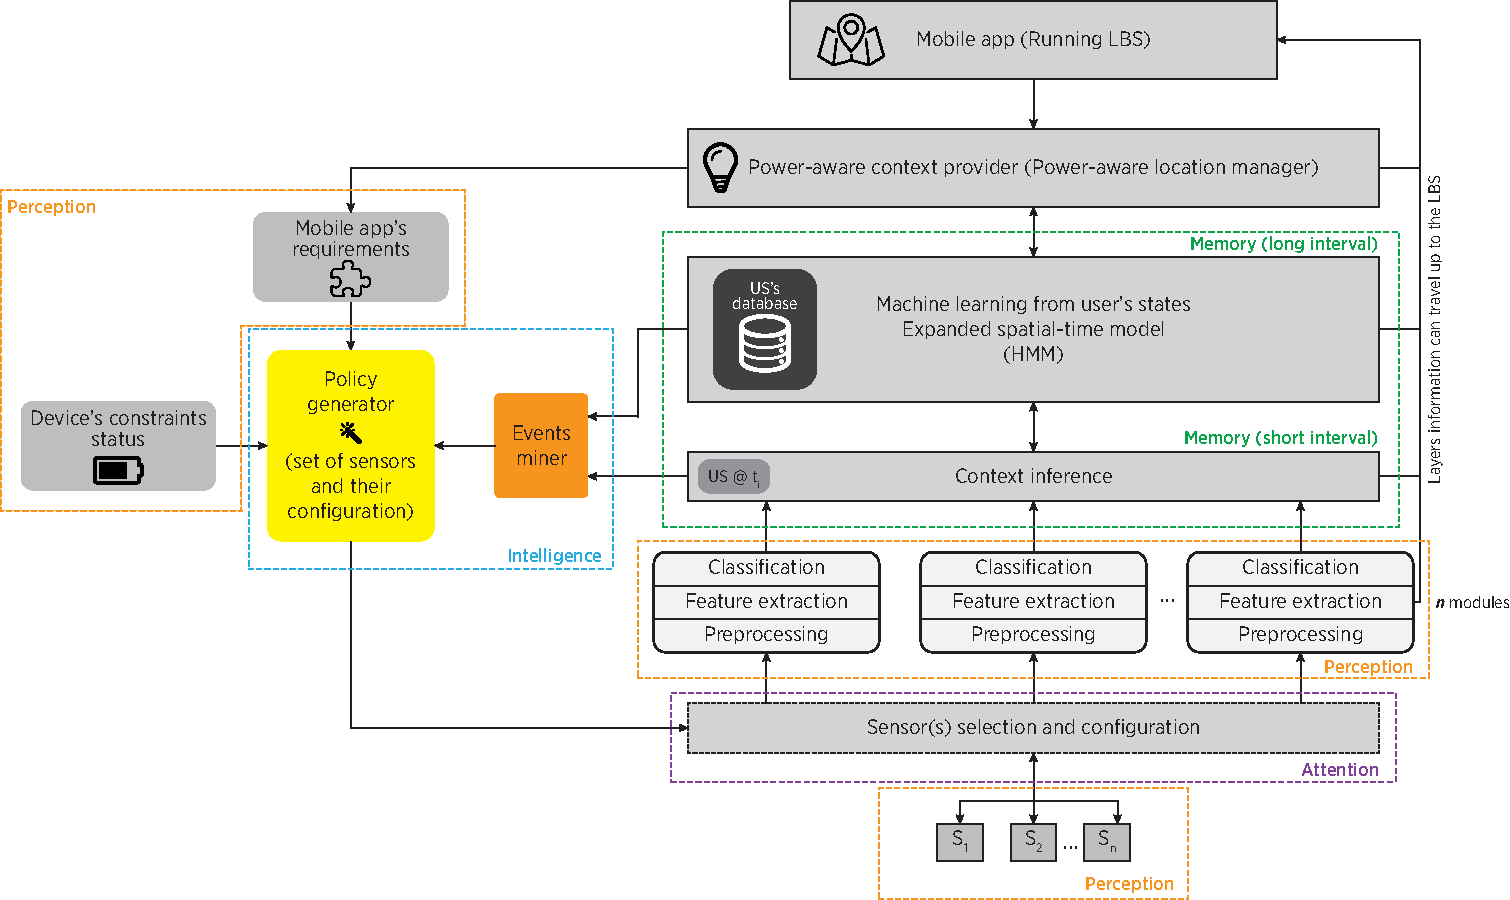
\includegraphics[width=\linewidth]{vectors/solution-general-overview}
  \caption{Conceptual solution}
  \label{fig:overall-architecture-of-proposed-system}
\end{figure}
\end{landscape}

Figure~\ref{fig:overall-architecture-of-proposed-system} shows the high-level architecture design of the proposed system solution.
At a first glance, the different components of a CDS can be identified, as well as the interaction between them.
There is an incremental processing of raw sensory data that starts on the different pipelines and ends up with its incorporation in the expanded spatial-time model and its notification to the running LBS.
Also, it could be observed the closed perception -- action cycle loop involving the perception of data from the environment, the associated processing (including memory) and the adaptation of actuation by using the intelligence-smart components.
Regarding this research work problems, the \emph{Perception} blocks (specially the sensor pipelines) are aimed at the problem of identifying mobility patterns, while the \emph{Intelligence} block maps to the problem posed by the generation of power-aware policies for sensors sampling.


As depicted by Figure~\ref{fig:overall-architecture-of-proposed-system}, the proposed system solution is composed by building blocks inspired on CDS, which interact only by passing message notifications as Event-Driven Systems do~\cite{Faison2011,Etzion2011}.
The step sequence of the perception -- action cycle of CDS is taken for describing the system components in the following paragraphs.

\subsubsection{Perception components}
The perception components of CDS are mapped into the following system solution components:
\begin{itemize}
  \item Hardware sensor listeners.
  \item Pipelines for classifying raw sensory data.
  \item Mobile application's requirements specification.
  \item Mobile device's constraints status (battery level).
\end{itemize}

\paragraph*{Hardware sensor listeners}
The raw sensory data supplied by sensors represents the raw material perceived by the smartphone from the environment.
Function callbacks are registered by the system solution in order to receive a message notification when sensors data has been collected.
Requests for sensors data are performed by the \texttt{Sensor(s) selection and configuration} block.

\paragraph*{Pipelines for raw data classification}
Hardly ever the incoming raw sensory data can be employed as is by further decision making components of a mobility analysis system.
There are two pipelines aimed at classifying GPS location and accelerometer data. 

The GPS pipeline detects stay points from the stream of location updates and also acts as a \texttt{Geofencing} unit that detects when user arrives and leaves a stay point.
The detection of stay points is performed through an event-driven adaptation~\cite{Perez-Torres2016b} of a GPS trajectory analysis algorithm~\cite{Li2008,Ye2009}, while the Geofencing task is achieved by contrasting each location update against the learned stay points information.
The adaptation of such algorithm is needed since typical trajectory analysis techniques are aimed at an off-line analysis, rather than at detecting stay points in an on-line manner.

The accelerometer pipeline features a HAR mechanism powered by a Naive Bayes classifier that analyses the stream of incoming accelerometer data~\cite{Torres-Huitzil2015} and identifies the activity performed by user within the set \{static, walking, running, vehicle\}.
Such HAR strategy was selected due to the reduced computation complexity of its classifier.
The raw data received by the pipeline is obtained through duty cycling of accelerometer.

Both pipelines generate a notification when any of the aforementioned mobility events (coarse and fine-grain) is detected.

\paragraph*{Mobile application's requirements}
The requirements of mobile application also represent relevant information that could impact on the behavior of system solution.
At the moment, the accuracy of the location tracking is the only requirement that the platform is designed to perceive.
The value of the accuracy parameter is discrete; a high accuracy requirement indicates that platform has to override many of its internal mechanisms for incrementing the sampling frequency of sensors.
A low accuracy requirement allows the platform to operate using all of its internal components and mechanisms, in particular the usage of memory information, producing higher power savings.

\paragraph*{Device's constraints status} 
Finally, the status of mobile device's constraints is a highly important factor that also impacts on the behavior of the system solution.
Once a notification of low battery level scenario is received, the platform perceives this as another notification and could reduce the access to sensors in order to make the most of the battery.
Such behavior could be overridden by the mobile application if energy is not a constraint and high accuracy is desirable.

\subsubsection{Memory components}
The system solution's memory components learn information about user mobility patterns.
The information learned is exploited for detecting when user arrives and/or leaves a stay point, so that the sensors usage could be adapted.
The working memory is composed by a 2-layer block that is fed with the outcome of the pipeline components.

\paragraph*{Context inference module (short interval memory)}
The first layer of memory is directly fed by the event notifications coming from mobility pipelines.
As such, it contains at any given moment the most recent user's mobility information, acting as a short interval memory that interprets what user is doing at the current moment.

\paragraph*{Expanded spatial-time model (long interval memory)}
It receives the context inference performed by the short interval memory, and builds a model of mobility composed by these inferences over a long time window.
The expanded spatial-time model then allows to identify a variety of mobility patterns information such as, the most important stay points in user mobility, the average commuting time between stay points, as well as a Hidden Markov Model (HMM) that explores the transition probabilities between stay points.

\subsubsection{The intelligence components}
All of the information acquired by the perception and memory components is delivered as event notifications to the intelligence components, which in turn adapt sensory operations according to such changes.
Recalling that the global objective of the system solution is to perform the location tracking of user, subject to the accuracy requirement and the battery level, the intelligence components handle the incoming high level information for producing a sensor management adaptation that reacts to mobility changes across time.

\paragraph*{Events miner}
The \texttt{Events miner} component explores the mobility learned and stored in both layers of memory for collecting meaningful information that could aid the adaptation of sensors operation.
As the \texttt{Event miner} can focus on specific memory information (rather than on the whole memory) it is said to exhibit attention capabilities and, in conjunction with memory layers, it acts as a pipeline dedicated to the retrieval and processing of memory information.
Among the information that could be extracted by the \texttt{Event miner} is:
\begin{itemize}
  \item The activity currently performed by user.
  \item The status of user mobility (inside a stay point or moving between stay points).
  \item The current stay point and/or the most likely stay point to be visited next.
  \item The visit frequency and weight of stay points in overall user mobility.
\end{itemize}
Depending on current mobility-context situation, this information could provide a valuable hint for adapting sensory operations.

\paragraph*{Policy generator}
The \texttt{Policy generator} is the holistic component that reunites all of the perception and memory information (which is explored by the \texttt{Events miner}) in order to make a decision for adapting sensory operations.
The time is a critical component in the operation of the \texttt{Policy generator}, as its outcome is dynamically adapted to changes in user mobility across time.

The changes in mobility and mobile device's constraints status are received as event-driven notifications, as well as those hints of mismatches between the mobility currently described by user and the mobility information learned by the expanded spatial-time model.
At any time, the \texttt{Policy generator} is able to explore memory information via the \texttt{Events miner} component for tuning its decision making.

The final outcome of \texttt{Policy generator} is a list of sensors (and associated configuration, i.e., the duty cycle) to employ in order to keep the user location tracking within mobile app's accuracy requirement and observing the current battery level.


\subsubsection{Attention components}
The system solution exposes two different cases of attention.
On the one hand, the \texttt{Events miner} component is able to focus on specific portions of memory, taking current time and context (user mobility state) as the filters to discard non-related data and provide only meaningful information to \texttt{Policy generator}.

On the other hand, the \texttt{Sensor(s) selection and configuration} block modifies the list of sensors to employ and their duty cycle, according to the specification provided by \texttt{Policy generator}.

In both cases, the system solution adapts the way on which its resources are managed.
In the case of memory, it only activates the right positions of memory useful for tuning sampling decision making, while in the case of sensors it dynamically selects and configure them according to changes observed in user mobility.




\subsection{An event-driven and cognitive implementation}
Although previous sections describe a conceptual event-driven solution inspired on CDS, it does not reflect many of its design details nor the specific tasks launched at every step of the perception -- action cycle.

A relevant aspect of the proposed system solution is the consideration of time as a key component, along with the mobility information itself.
Time allows the platform to learn mobility information, with the memory components acting as an additional pipeline of time.
Similarly, time allows to dynamically adapt sensory operations according to changes detected in user mobility.
As a result, one of the main contributions of the proposed approach is to go beyond typical and static machine learning strategies employed in literature, and favor the insight of an autonomous system on which an infinite loop featuring learning and exploring attributes with self-feedback information is the core engine.

Having the cognitive feature as one of its most important characteristics, Figure~\ref{fig:smartness-components} depicts a more comprehensive description of the interaction of platform components and presents a zoom-in of the tasks performed in the \texttt{Policy generator}, now highlighted inside the \texttt{Cognitive control} block.
Also the notion of different types of memory is represented by the figure.
Next sections focus on the description of the memory and cognitive tasks executed by the proposed system solution.


\subsubsection{Memory processing throughout the system solution}
As described in Section~\ref{sec:theoretical-framework}, CDS hold different types of memory across their components.
Their usage and implementation in the system solution are described as follows.

\paragraph*{Perceptual memory} 
The perceptual memory is employed in the \textbf{Perception} block, as it allows to associate or map incoming sensors stimuli to observations made in the past.
In this way, the platform can actually observe what is happening in the environment, in this case the mobility described by user, and generate a message notification when an interesting event is discovered.

The \texttt{HAR module} is powered up by a Naive Bayes classifier, which acts as a perceptual memory element that once trained identifies the fine-grain mobility pattern (i.e., activity) performed by user.

Perception components are not strictly required to employ a typical classification algorithm to be considered as such.
The \texttt{Mobility Analyzer} is composed by the \texttt{Stay points detector} and \texttt{Geofencing} blocks, and it directs to them each location update right after its reception.
The \texttt{Stay points detector} uses the previously described event-driven trajectory analysis algorithm for conducting an on-line detection of frequent places in user mobility.
The perceptual memory in the \texttt{Mobility Analyzer} is carried out by the \texttt{Geofencing} component, which determines whether the location updates represent an arrival or departure from a stay point, generating an event-driven notification for such situations (there is also a notification generated for the case a location update does not produce any mobility changes).

Finally, it is important to recall that perception could also hold a window of past perceived stimuli, and use such information for improving the accuracy of its outcome (represented as the \texttt{Perceptor memory} block).
For instance, a single location update is not enough for determining an arrival to a stay point, as user could have only passed by a frequent location (but not entering to it).
In this case, several location fixes observed recently and time information could aid the Geofencing mechanism for detecting arrivals accurately.


\paragraph*{Working memory}
The working memory in the system solution is mainly represented by the expanded spatial-time model.
On such model, the information learned from sensory data collected in a long time window interval is analyzed and stored.
The time window length is within the granularity of a week, distinguishing between weekdays (Monday to Friday) and weekends (Saturday and Sunday).
The core of the expanded spatial-time model is an HMM that holds the transition probabilities for traversing between stay points.
Nonetheless, the information is enriched with time-dimension aspects, like the average arrival and departure times; activity aspects, like the transportation mode used for moving between stay points; and the ability to increase or decrease the importance of learned stay points across time (hence the \emph{expanded} attribute). 

This last feature refers to the mobility changes that user could describe across time; for instance, when user gets a new job, the new stay point will appear on its associated mobility model, while the previous job's stay point will \emph{fade out} when time passes.
As a result, the long-term memory information is updated right after each mobility event notification is received.

Besides the long-term memory represented by the expanded spatial-time model, the working memory also comprises information related to current time, i.e., short time window information.
This information has a shorter life span, as it is updated when new mobility event notifications are received, replacing the existing ones. 

As it has been mentioned, the \texttt{Events miner} has the ability to explore the short and long-term memory information, in order to deliver on-demand data requested by the \texttt{Policy selector} component.

Finally, one relevant aspect of the working memory in the proposed platform, is that the incorporation of incoming mobility event notifications, performed by the \texttt{Memory mediator} component, is followed by a mismatch identification process, on which the discrepancies between currently observed data and the learned information are detected and notified to the \texttt{Cortex} component.
This allows the platform to react to situations that are likely to represent changes in user mobility.

\paragraph*{Executive memory}
As it will be described later on in further sections, the \texttt{Sampling decision maker} is the element that actually instructs which sensors and how they should be configured for conducting the next perception -- action cycle.

This final command is influenced by decisions and historical information generated in previous perception -- action cycles, denoted as the $Z^{-1},Z^{-2},\ldots,Z^{-n}$ buffer in Figure~\ref{fig:smartness-components}.
Even though mobility information currently observed by sensors could represent a specific sampling decision, the executive memory allows to observe the consequences of past decisions and rely on such gained information for fine tuning of sensory operations.


\subsubsection{Cognitive components of the system solution}
From the CDS characteristics of the proposed system solution, the perception, action, memory, and attention have been described in previous sections.
Nonetheless, the intelligence attribute has been only described from the perspective of the influence of time on its behavior.

The core-engine of the system solution is depicted by the \texttt{Cognitive control} meta-block of Figure~\ref{fig:smartness-components}.
Such meta-block is represented by the \texttt{Policy generator} component in Figure~\ref{fig:overall-architecture-of-proposed-system}, but in this description a zoom-in of the component is given, highlighting how it is implemented and the different tasks that internal modules have to accomplish.
As the holistic component of the system solution, the \texttt{Cognitive control} meta-block manages information coming from perception and memory components, and it holds the most important role of the platform for adapting attention focus in terms of how sensory operations must be performed.

The specific event-driven operation of the \texttt{Cognitive control} meta-block is as follows.
First, the perception components notify to \texttt{Working memory} the mobility changes events.
After incorporation in memory, the Working Memory notifies to the \texttt{Cognitive control} about changes and the possible mismatches found between sensors data and learned information.
In particular, the \texttt{Events Miner} receives these notification events and disseminate them to other \texttt{Cognitive control} components.

Upon reception of mobility events, the \texttt{Policy selector} looks into a \texttt{Pool of explore-exploit policies}, for filtering those policies that could be employed for modifying sensors access according to current context information.
The \texttt{explore} policies of the pool refer to those that can be employed by the system when learning mobility patterns. 
Broadly speaking, the explore policies represent a high sampling frequency of sensors in order to carry out the learning process.
On the contrary, the \texttt{exploit} policies are employed when the system solution has learned mobility information and must employ it for adapting the sampling frequency and produce power savings.

The \texttt{Policy selector} is able to solicit memory information by on-demand request to the \texttt{Events miner} for incrementing its awareness about long-term information, or for further clarification about detected mobility mismatches.
The selected policies are notified to the \texttt{Sampling decision maker}.

Simultaneously, the \texttt{Events miner} also provides information to the \texttt{Sampling decision maker} about mobility states and decisions taken in previous perception -- action cycles.
This allows the platform to pre-adapt to mobility changes that user could be describing in real world\cite{Haykin2014}.
For instance, a list of mobility states that indicate a reduction in user speed (the sequence of \texttt{vehicle, walking} activities) could represent that the next state will be the user stationery, information that could aid the adaptation of sensory operations for the next cycle.

The \texttt{Sampling decision maker}, upon reception of both filtered policies and information of past decisions and experiences, defines the list of sensors and associated configuration for providing location tracking services with a reduced energy consumption and within the mobile app's accuracy requirement.
Internally, the \texttt{Sampling decision maker} selects the policy that best fits with the current mobility information as well as with the previous sampling decisions (experiences).
As a result, the \texttt{Sampling decision maker} involves both levels of memory (long and short term), the inferences made upon them, the mobile app's accuracy requirements and the status of mobile device's constraints.
The battery status has a high impact on decision making, in such a way that a low energy scenario could override the internal self-adaptive sampling mechanisms and directly select a policy for reducing sampling frequency and making the most of battery.

The outcome of the \texttt{Sampling decision maker} is directed as feedback information to the \texttt{Events miner}, which incorporates it in the executive memory for tuning the decision of next perception-action cycle.
The feedback information is composed by the mobility pattern detected, the selected policy and its parameters.

Finally, such outcome is also employed for focusing the attention of the platform in the next relevant mobility events to be detected.
Therefore, the decision is then materialized as a list of sensors to employ in the next cycle (including the associated configuration), which is notified to the \texttt{Actuation} block.

The \texttt{Actuation} block isolates all of the technical barriers, such as the management of power states of the mobile platform, and instructs sensors hardware to perform the sampling as specified by the \texttt{Sampling decision maker}.
At this point, the current perception-action cycle is completed and the next one is started once the next mobility events are generated.

\begin{landscape}
\begin{figure}
  \centering
  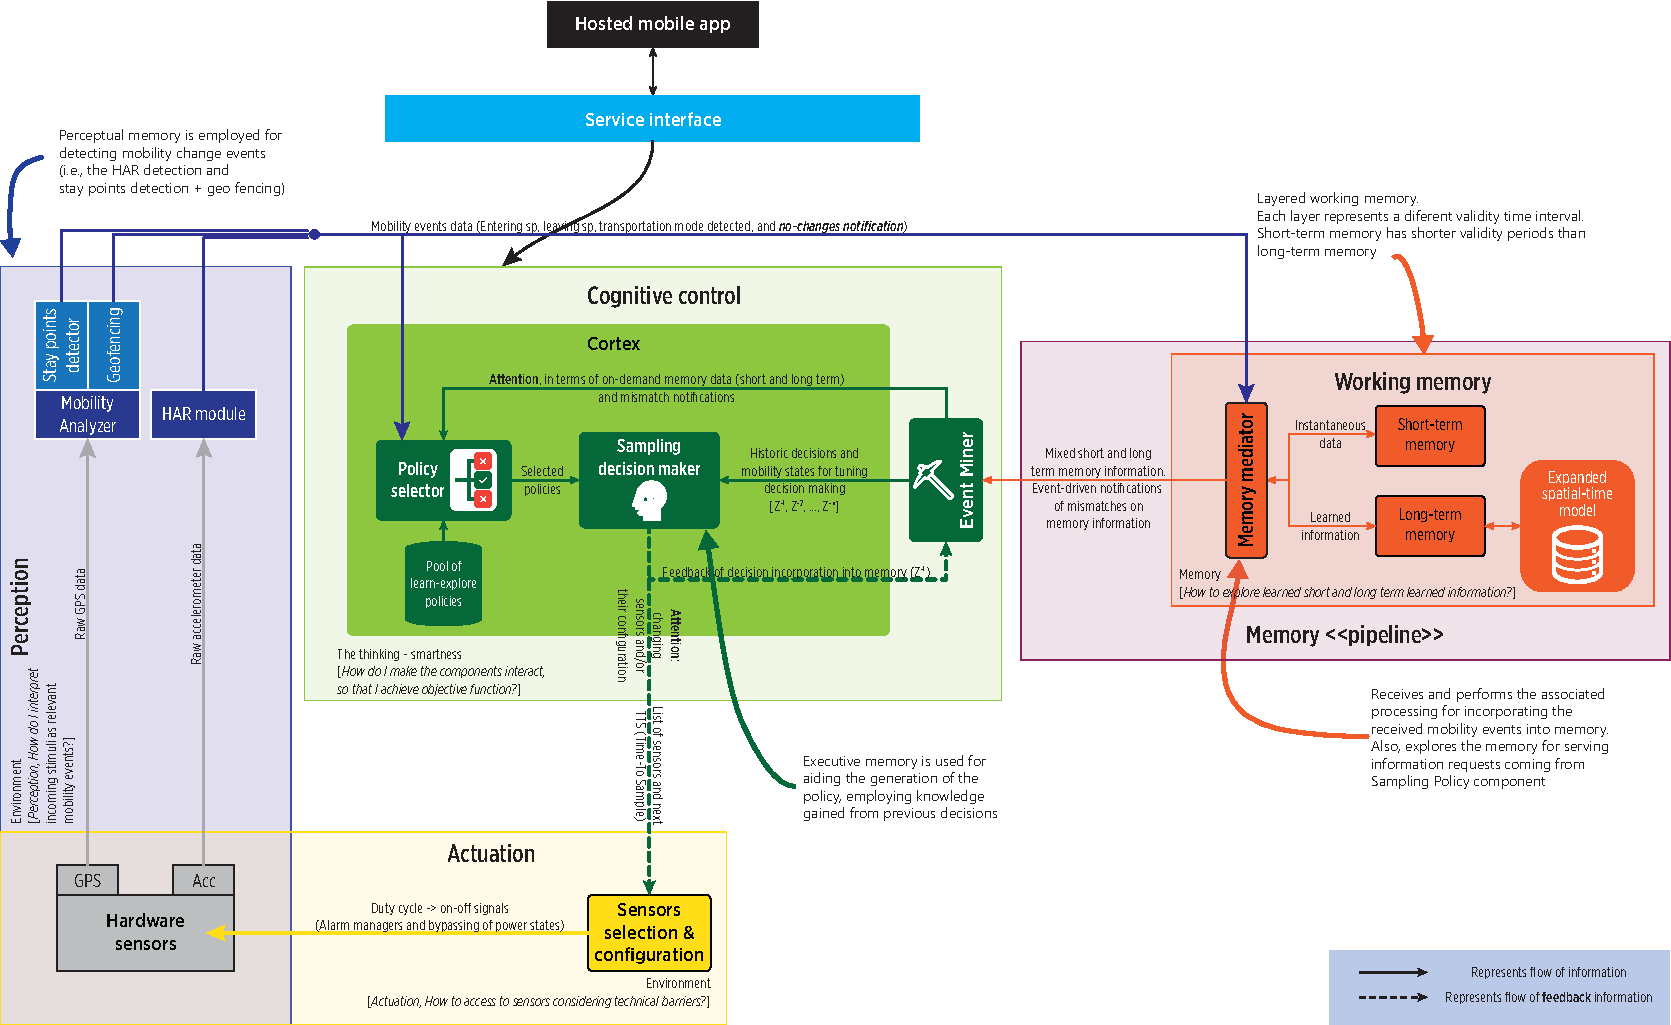
\includegraphics[width=\linewidth]{vectors/smartness-components-v4}
  \caption{Cognitive components of system solution and their interaction.}
  \label{fig:smartness-components}
\end{figure}
\end{landscape}




 
%                                                                                                                                                             
%     .oPYo.                                       o                                o             8                                          8     o           
%     8.                                                                            8             8                                          8     8           
%     `boo     `o  o'   .oPYo.   .oPYo.   oPYo.   o8   ooYoYo.   .oPYo.   odYo.    o8P   .oPYo.   8       oPYo.   .oPYo.   .oPYo.   o    o   8    o8P   .oPYo. 
%     .P        `bd'    8    8   8oooo8   8  `'    8   8' 8  8   8oooo8   8' `8     8    .oooo8   8       8  `'   8oooo8   Yb..     8    8   8     8    Yb..   
%     8         d'`b    8    8   8.       8        8   8  8  8   8.       8   8     8    8    8   8       8       8.         'Yb.   8    8   8     8      'Yb. 
%     `YooP'   o'  `o   8YooP'   `Yooo'   8        8   8  8  8   `Yooo'   8   8     8    `YooP8   8       8       `Yooo'   `YooP'   `YooP'   8     8    `YooP' 
% :::::.....:::..:::..::8 ....::::.....:::..:::::::..::..:..:..:::.....:::..::..::::..::::.....:::..::::::..:::::::.....::::.....::::.....:::..::::..::::.....:
% ::::::::::::::::::::::8 :::::::::::::::::::::::::::::::::::::::::::::::::::::::::::::::::::::::::::::::::::::::::::::::::::::::::::::::::::::::::::::::::::::
% ::::::::::::::::::::::..:::::::::::::::::::::::::::::::::::::::::::::::::::::::::::::::::::::::::::::::::::::::::::::::::::::::::::::::::::::::::::::::::::::
\section{Experimental results}\label{sec:experimental-results}
The proposed system solution has been implemented as an event-driven middleware for the Android platform, and it is able to provide location tracking services to subscribed mobile applications.

Several technical barriers had to be overcome, most of them referring to the management of smartphone's power states.
Additionally, a proper employment of the mechanisms provided by Android SDK was needed, so that the scheduling of sensor sampling could be achieved, regardless of current power state and the level of interaction of user with the mobile app~\cite{Perez-Torres2016b,Android2016b}.
Different workarounds were needed depending on the version of the Android mobile OS, as newer versions incorporate out-of-the-box aggressive power management strategies for reducing energy consumption.

Several experiments have been carried out at different stages of the proposed system solution, each of them with specific purpose.
The first and second experiments, described later on in this section, were performed using the proposed platform implementing only basic aspects of the perception-action cycle, disregarding the usage of any adaptive sampling policy.
In the case of the third experiment, the platform incorporates a basic sampling decision maker that follows a policy for selecting a different sampling period depending on whether user is inside a stay point or describing motion during a trajectory.

For all of the experiments, the smartphones employed were two Google Nexus 6 units, featuring a 2.7 GHz quad-core processor, 3 GB RAM, and a new 3220 mAh battery, running Android 6 (Marshmallow).
Each round of the experiments involved the carrying of the two smartphones by a campus student, together with a Qstarz BT-Q1000eX GPS logger (acting as a ground-truth GPS data collector) with a sampling frequency of 1 Hz.
Similarly, for all of the experiments, the parameters for the proposed event-driven stay points detection algorithm were 500m for the size of geographical area and 45 minutes for minimum time size.
Further details and results of experiments are presented in next sections.


\subsection{Feasibility of running a mobility analyzer fully on-device}
The first experiment was aimed at validating the feasibility of having a mobility analyzer platform running entirely on the mobile device, subject to different stress levels, without the need for computational offloading unlike other Mobile Cloud Computing (MCC) oriented solutions\cite{Perez-Torres2016b}.

In this context, the feasibility is understood as the ability for executing the middleware in the mobile device under different stress levels without a premature finalization caused by CPU and memory consumption usage issues.

A couple of sample LBS mobile apps where developed, and each of them requested location updates to the developed middleware.
The referred stress levels were implemented by the sampling periods in the set \{30, 60, 90, 120, 150 seconds\}, which produce different workloads in the CPU, memory, and battery consumption of the smartphone.

Each of the smartphones executed an event-driven variant of an off-line stay points detection algorithm~\cite{Li2008,Ye2009,Perez-Torres2016b}.
The only difference between the two variants, \texttt{buffered} and \texttt{sigma}, relies on how location data is incorporated in the processing.
The buffered version maintains a sublist of GPS fixes in memory that might eventually be transformed in a stay point.
On the other hand, the sigma version only accumulates the latitude and longitude values of each location fix, reducing memory requirements.


\begin{table}
\centering
\caption{Summary of results of first experiment (SP = stay point).}
\label{tbl:experiment-1}
\resizebox{0.68\textwidth}{!}{%
\begin{tabular}{@{}ccccc@{}}
\toprule
\textbf{\begin{tabular}[c]{@{}c@{}}Sampling\\ period  (seconds)\end{tabular}} & \textbf{\begin{tabular}[c]{@{}c@{}}Event-driven\\ algorithm\end{tabular}} & \textbf{\begin{tabular}[c]{@{}c@{}}Obtained\\ GPS fixes\end{tabular}} & \textbf{\begin{tabular}[c]{@{}c@{}}Average GPS\\ fixes per SP\end{tabular}} & \textbf{\begin{tabular}[c]{@{}c@{}}Running time \\ (minutes)\end{tabular}} \\ \midrule
\multirow{2}{*}{30} & Buffered & 3,876 & 218.3 & 6,752 \\
 & Sigma & 5,199 & 244.4 & 8,243 \\
 \cmidrule{2-5}

\multirow{2}{*}{60} & Buffered & 5,307 & 155.6 & 14,877 \\
 & Sigma & 3,054 & 126.3 & 8,428 \\
 \cmidrule{2-5}

\multirow{2}{*}{90} & Buffered & 2,573 & 115.2 & 7,694 \\
 & Sigma & 2,447 & 108.1 & 7,522 \\
 \cmidrule{2-5}

\multirow{2}{*}{120} & Buffered & 1,708 & 77.4 & 8,460 \\
 & Sigma & 1,993 & 82.2 & 10,214 \\
 \cmidrule{2-5}

\multirow{2}{*}{150} & Buffered & 1,417 & 53.8 & 10,433 \\
 & Sigma & 1,651 & 51.1 & 10,349 \\
 \bottomrule
\end{tabular}%
}\end{table}

The results of the first experiment are summarized in Table~\ref{tbl:experiment-1}.
The column \emph{sampling period} indicates the sampling period employed for accessing the GPS receiver, while the \emph{algorithm variant} column indicates the version of the algorithm executed by the mobile device.
Column \emph{obtained GPS fixes} refers to the amount of GPS fixes that were requested by the middleware to the mobile OS and that were actually obtained.
It is important to mention that a 1 minute timeout interval was established for obtaining each location fix; if the timeout was reached, the GPS location fix was considered not valid and a new GPS reading was scheduled.
The column \emph{average GPS fixes per SP} indicates the average amount of location fixes involved in all of the calculated stay points.
Such amount gives an idea of the amount of memory that the smartphone should manage for executing the \emph{buffered} algorithm variant.
Finally, the \emph{running time} indicates how long (minutes) the experiment was executed by the smartphones, starting from a full-charged battery and ending with a 4\% battery level (such battery level was employed so that the last stay point could be calculated before the smartphone was shut down due to battery depletion).

For all of the sampling periods, both smartphones were able to calculate stay points without being affected by their memory and computing capabilities, ensuring its feasibility.
By analyzing the performance of each algorithm during the trials, it is noteworthy that the usage of larger sampling periods incremented the total running time of each trial, with the exception of the outlier represented by the \emph{buffered} version with the \emph{60 seconds} sampling period, which describes a running time even higher than the obtained in the \emph{150 seconds} sampling trial.
Such outlier could be caused by the multiple background tasks that smartphones perform and that affect the transitions to the different internal power states of the mobile platform.
Similarly, as could be intuitively inferred, shorter sampling periods could obtain higher amounts of GPS fixes in each algorithm variant, again with the same outlier of \emph{60 seconds} sampling trial.
Also, it is noteworthy that the \emph{running time} does not exactly correspond to \emph{obtained GPS fixes} $\times$ \emph{sampling period} value since each fix is not obtained immediately and because of the aggressive internal mechanisms that the Android OS implements for reducing energy consumption in the smartphone's idle state like the \emph{doze} and \emph{app standby} features~\cite{Android2016b}.


\subsection{Evaluation of energy consumption of on-device solution vs. offloading approach}
The energy consumption of the proposed system solution was also evaluated against a MCC oriented solution, which also requested location updates to the developed middleware but offloaded its processing to an external server via mobile data network.
The same sampling periods and smartphone units of previous experiment were employed.


\begin{table}
\centering
\resizebox{\textwidth}{!}{%
\begin{tabular}{@{}cccccccc@{}}
\toprule
\textbf{\begin{tabular}[c]{@{}c@{}}Sampling\\period\\(seconds)\end{tabular}}  & \textbf{\begin{tabular}[c]{@{}c@{}}Processing\\ strategy\end{tabular}} & \textbf{\begin{tabular}[c]{@{}c@{}}Obtained \\ GPS fixes\end{tabular}} & \textbf{\begin{tabular}[c]{@{}c@{}}GPS-on time\\ (minutes)\end{tabular}} & \textbf{\begin{tabular}[c]{@{}c@{}}Average \\ acquisition \\  time per fix\\ (seconds)\end{tabular}} & \textbf{\begin{tabular}[c]{@{}c@{}}Running time\\ (minutes)\end{tabular}} & \textbf{\begin{tabular}[c]{@{}c@{}}Data sent\\ (bytes)\end{tabular}} & \textbf{\begin{tabular}[c]{@{}c@{}}Data received\\ (bytes)\end{tabular}} \\ \midrule

\multirow{2}{*}{30}  & On-device   &  12,341 & 1,614 & 7.84  & 7,790 & - & - \\
                          & MCC oriented &  9,324 &   770 & 4.98  & 5,402 & 1,084,901 & 18,796 \\
\cmidrule(l){2-8}
\multirow{2}{*}{60}  & On-device    & 10,816 & 1,219 & 6.76 & 12,028 & - & - \\
                          & MCC oriented &  7,205 &   764 & 6.45 &  7,907 & 838,640 & 14,696 \\
\cmidrule(l){2-8}
\multirow{2}{*}{90}  & On-device    & 7,868 & 1,178 & 8.91 & 13,075 & - & - \\
                          & MCC oriented & 5,624 &   546 & 5.84 &  8,946 & 653,833 & 12,223 \\
\cmidrule(l){2-8}
\multirow{2}{*}{120} & On-device    & 5,189 & 809 & 9.26 & 11,289 & - & - \\
                          & MCC oriented & 4,332 & 387 & 5.43 &  8,931 & 504,012 & 8,838 \\
\cmidrule(l){2-8}
\multirow{2}{*}{150} & On-device    & 5,576 & 933 & 9.94 & 14,998 & - & - \\
                          & MCC oriented & 4,564 & 452 & 6.06 & 11,619 & 530,764 & 10,309 \\
\bottomrule
\end{tabular}%
}
\caption{Summary of results of second experiment.}
\label{tbl:experiment-2}
\end{table}


The results of the experiment are summarized in Table~\ref{tbl:experiment-2}.
The \emph{GPS-on time} column refers to the estimated effective time (minutes) that the GPS receiver was turned on for acquiring location fixes.
The column \emph{average acquisition time per fix} indicates the average amount of seconds invested for acquiring each location fix, which is calculated as the quotient between GPS-on time and the amount of obtained GPS fixes.
Finally, the \emph{data sent} and \emph{data received} columns, applicable only to the MCC oriented tests, include the total amount of bytes requested by the mobile app to be sent as payload and the total amount of bytes received as payload in the smartphone by the server side, respectively.

From these results, it could be observed that all of the local executions, regardless of the employed duty cycle, outperform the running time of the corresponding remote trials, increasing the battery lifetime in factors within the range 1.26 to 1.52\textbf{x}.
This produces a more efficient usage of energy resources and allows to conduct location tracking and stay points detection for a longer time.
On the other hand, the MCC oriented strategies achieve shorter running times and obtain a lower amount of GPS fixes than corresponding local trials, which is caused by the energy overhead generated by the data transmission that contributes to a faster depletion of battery.
It is also worth to note how the average time for obtaining a fix in the local trials is increased when longer sampling periods are employed, which could be explained by the different types of power states in the operation of GPS receiver (cold-start, hot-start, and warm-start).
Longer sampling periods might represent a heavier energy demand since GPS receiver should perform a cold-start for obtaining a GPS fix.
The average acquisition time of GPS fixes in the MCC oriented implementations is lower than the on-device strategy, which is attributable to the assistance provided by the mobile data network to the A-GPS receiver of the smartphone~\cite{Agarwal2002,Liu2012}.
However, energy savings are still offered by on-device stay point detection when increasing the underlying sampling interval.
% TODO acercar colocar en trabajo futuro: In this regard, a power-aware middleware for location tracking might leverage on these equivalences for achieving an adaptive sampling that ensures accuracy without jeopardizing energy resources.

\begin{figure}
  \centering
  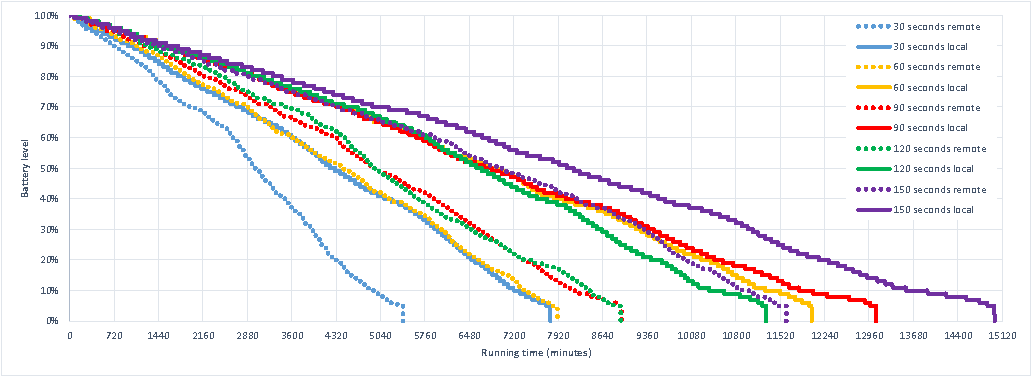
\includegraphics[width=\columnwidth]{vectors/plot-energy-performance-r2}
  \caption{Energy performance comparison of on-device vs. MCC oriented sample apps using different GPS sampling periods.}
  \label{fig:plot-energy-performance}
\end{figure}

Figure~\ref{fig:plot-energy-performance} shows the energy consumption performance across time of both strategies for all of the employed sampling periods.
The results shown on the plot were mapped to a sampling-independent timing format where the elapsed time from the beginning of the experiment was considered for evaluation and representation.
As it could be expected, shorter GPS sampling periods have a higher impact in battery performance, which reduces its level quicker than longer sampling periods.
Note also that for all cases the MCC oriented solutions produce a higher battery consumption than their on-device equivalent.
In particular, it could be observed from the plot how the different tests corresponding to remote versions are finished in almost a sequential order (i.e., trials end in ascending order of its sampling period) with the exception of the \emph{120 seconds} test, which ends very close to the \emph{90 seconds} trial, but 15 minutes before.
In the case of the local tests, a similar situation is found, where tests end following an increasing order of their sampling period, again with the exception of the \emph{120 seconds} sampling trial that finishes 739 minutes before the \emph{60 seconds} trial.
The unexpected early finalization of the \emph{120 seconds} trials, both in remote and local tests, suggests that this specific sampling period could represent a breaking point in the operation of the GPS receiver of the employed smartphones.
A pragmatic interpretation is that location update requests in a \emph{120 seconds} sampling period produce cold and/or warm starts in the operation of GPS receiver.
% A pragmatic interpretation is that the operation of the GPS receiver produces cold and/or warm starts once each individual location request is received in a \emph{120 seconds} sampling period.
This means that for some of the sampling periods, the ephemeris and almanac information of GPS satellites must be updated, producing an additional energy overhead that increases energy consumption, up to the point of finishing the execution of the trial even before than shorter sampling periods.

From the results of the second experiment, we find out a tendency recalling the power benefits of the proposed on-device middleware.
However, these results can not be generalized to other scenarios considering different mobility patterns.
In order to have further insight into energy gain factors, more experimental trials are needed so that a better explanation of the battery depletion in function of the different sampling periods, mobility of user, and underlying technical aspects could be given.
%It is noteworthy the existence of issues related to the accuracy of GPS fixes obtained by the smartphone.
%Because of these issues, some stay points were prematurely calculated, as the reported GPS fixes described changes in the location that were considered as the user leaving a stay point.
Nonetheless, as the experimentation's results show, there is room for producing power savings by means of a policy manager that could adapt the duty cycle of the GPS receiver and at the same time, obtain an accurate location tracking of user, as is shown in~\cite{Paek2010,Lu2010,Chon2014}.
%Such adaptive duty cycling scheme could be based on context data coming from different sensors as well as from information extracted by machine learning techniques that would allow to make predictions about user mobility.

\subsection{Evaluation of integral middleware solution} 
The purpose of this experiment was to perform an initial integral test of the whole functionality of the platform, involving the perception-action cycle (the \texttt{StayPoint detector} and \texttt{Geofencing} modules), the attention capabilities, the memory learning (short and long time intervals), as well as the decision making for adapting sensors sampling.
An additional motivation for this trial was the collection of mobility data for designing sampling policies that could perform an accurate learning of stay points, and a reliable identification of visits to them.

Depending on the current mobility state described by user, the \texttt{Sampling decision maker} selects a different duty cycle scheme for accessing GPS receiver and accelerometer.
In the case of the \texttt{onTrajectory} state, the decision maker selects a high frequency sampling period of 30 seconds.
For the case of \texttt{onStayPoint} mode, the decision maker implements a lower sampling period of 120 seconds (2 minutes).
% Two pairs of smartphones were employed, the same Nexus 6 smartphones and two Samsung Galaxy Note II units, featuring a 1.6 GHz quad-core processor, 2 GB RAM, and a 3100 mAh battery, running Android 4.4.2 (JellyBean).

% Such sampling policy was implemented in a smartphone, while the other unit implemented a fixed sampling period of 30 seconds, regardless of current mobility state.
Such sampling policy was implemented in a smartphone, and the experimentation was launched having the platform memory empty.
Another implementation of a fixed sampling period of 30 seconds, regardless of current mobility state, was also tested with the purpose of energy consumption comparison.
The spatial and time summary of this experiment results are shown in Table~\ref{tbl:space-time-summary}.
Table~\ref{tab:stay-points-weights} presents a snapshot of the different stay points learned by the platform, including its weight and visits information.

\begin{table}
\centering
\resizebox{0.84\textwidth}{!}{%
\begin{tabular}{@{}lrlr@{}}
\toprule
\multicolumn{2}{c}{\textbf{Space information}} & \multicolumn{2}{c}{\textbf{Time information}}                \\ \midrule
Total fixes                       & 4,719    & Total time (minutes)            & 8,848.56                     \\
Fixes inside stay points (94.3\%) &  4,451   & Total stay points time (96.4\%) & 8,526.45                     \\
Fixes on trajectory (5.7\%)       & 268      & Total trajectory time  (3.6\%)  & 322.11                       \\
Detected stay points              & 6        & Semantic time duration          & Tuesday night - Monday night \\
Total trajectories                & 28       &                                 & (approximately 6 days)       \\ \bottomrule
\end{tabular}%
}
\caption{Space and time summary of mobility information}
\label{tbl:space-time-summary}
\end{table}

\begin{table}
\centering
\resizebox{0.8\textwidth}{!}{%
\begin{tabular}{@{}rlrrrr@{}}
\toprule
\multicolumn{1}{c}{\textbf{\#}} & \multicolumn{1}{c}{\textbf{Semantic}} & \multicolumn{1}{c}{\textbf{Visit count}} & \multicolumn{1}{c}{\textbf{Stay time (minutes)}} & \multicolumn{1}{c}{\textbf{Absolute weight}} & \multicolumn{1}{c}{\textbf{Relative weight}} \\ \midrule
1 & Park & 3 & 254 & 2.88\% & 2.99\% \\
2 & Home & 8 & 5,767 & 65.18\% & 67.64\% \\
3 & Cinvestav & 5 & 2,090 & 23.62\% & 24.51\% \\
4 & Fast food & 6 & 78 & 0.89\% & 0.92\% \\
5 & Bob's home & 6 & 260 & 2.94\% & 3.05\% \\
6 & Coffee shop & 1 & 75 & 0.85\% & 0.89\% \\ \bottomrule
\end{tabular}%
}
\caption{Stay points weights and visits information}
\label{tab:stay-points-weights}
\end{table}

These results allow to obtain a preliminary vision of the mobility information that could be obtained and exploited when using GPS data.
Although the employed sampling policy is implemented through fixed sampling periods, they are chosen when the platform switches between mobility modes, an operation that can be performed only if the platform has learned stay points information properly.

Also, the usage of such simple sampling policy shows the possibility of producing a more efficient usage of energy resources.
Figure~\ref{fig:energy-performance-early-integral-test} shows the energy consumption across time of both implementations.
Note that at the beginning of the test (around 24 hours) the energy consumption rate is similar.
Nevertheless, after this point the energy consumption of the 30 seconds - 120 seconds scheme reduces the discharging rate of battery.
This situation occurs because at that time the platform has learned the most important stay points (\emph{Home and Cinvestav}), and the subsequent visits allowed the platform to reduce the sampling frequency.

 \begin{figure}
  \centering
  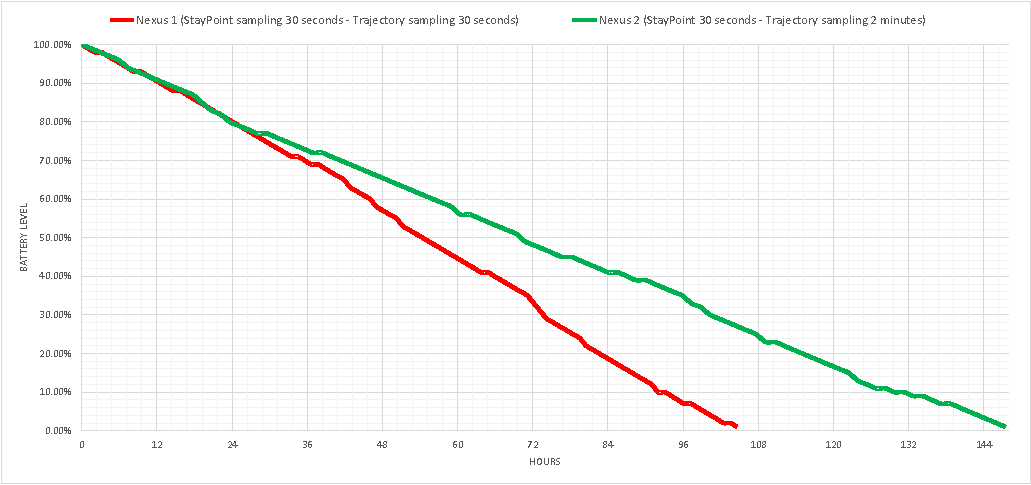
\includegraphics[width=\columnwidth]{vectors/energy-performance-early-integral-test}
  \caption{Energy performance of fixed sampling period vs. simple sampling policies. Battery lifetime increase of 1.41\textbf{x} (42.8 hours)}
  \label{fig:energy-performance-early-integral-test}
\end{figure}

From these results, it could be identified the opportunity for further reduction of energy consumption.
Intuitively, such reduction could be obtained if a more aggressive policy is implemented when user is inside the stay points with the larger weight.
The sampling scheme could be guided by the stay time information learned in the expanded spatial-time model.
Similarly, a more efficient sampling scheme could be employed in the \texttt{onTrajectory} mode, aided by activity information detected from accelerometer data.




 
%                                                                                               
%      ooooo              o                                                               8      
%      8                  8                                                               8      
%     o8oo     o    o    o8P   o    o   oPYo.   .oPYo.       o   o   o   .oPYo.   oPYo.   8  .o  
%      8       8    8     8    8    8   8  `'   8oooo8       Y. .P. .P   8    8   8  `'   8oP'   
%      8       8    8     8    8    8   8       8.           `b.d'b.d'   8    8   8       8 `b.  
%      8       `YooP'     8    `YooP'   8       `Yooo'        `Y' `Y'    `YooP'   8       8  `o. 
% :::::..:::::::.....:::::..::::.....:::..:::::::.....:::::::::..::..:::::.....:::..::::::..::...
% :::::::::::::::::::::::::::::::::::::::::::::::::::::::::::::::::::::::::::::::::::::::::::::::
% :::::::::::::::::::::::::::::::::::::::::::::::::::::::::::::::::::::::::::::::::::::::::::::::
\section{Future work}\label{sec:future-work}
As described in previous section, the feasibility of the running the proposed system solution in a constrained mobile device, and the energy improvements over a MCC oriented solution have been demonstrated by specific experimentations.
The third experiment allowed to start the collection and analysis of mobility information using all of the components of the proposed solution.
Such experiment also tested a simple decision maker for adapting sampling frequency that reduced the energy consumption when compared against a fixed sampling.
However, more work is needed for improving policies generation according to what the platform is able to perceive from the environment, and its analysis against learned information.
In accordance to proposed methodology, the next tasks have been identified for the following year:
\begin{itemize}
  \item Continue the data collection using the platform for further analysis.
  \item Select and delimiting mobility scenarios that could represent a challenge for the mobile platform.
  For instance, how to difference if user actually enters a stay point from a user only passing by near a stay point.
  \item Launch experiments targeted to such scenarios for analyzing what the platform perceives.
  \item Design and generate policies that represent behaviors aimed at these mobility scenarios.
  \item Launch experiments for validating the generated policies.
\end{itemize}

Additionally, for mid-term, it is needed to perform a full-integral evaluation of the platform, including the generated policies.
This evaluation will be performed in terms of energy consumption and the time-spatial accuracy of the location tracking (both at stay points and trajectory modes).
Such tasks, as a single unit, are aimed at defining policies towards adaptive sampling, which could further reduce the energy consumption of the proposed solution.




%                                                                                          
%     .oPYo.                             8                      o                           
%     8    8                             8                                                  
%     8        .oPYo.   odYo.   .oPYo.   8   o    o   .oPYo.   o8   .oPYo.   odYo.   .oPYo. 
%     8        8    8   8' `8   8    '   8   8    8   Yb..      8   8    8   8' `8   Yb..   
%     8    8   8    8   8   8   8    .   8   8    8     'Yb.    8   8    8   8   8     'Yb. 
%     `YooP'   `YooP'   8   8   `YooP'   8   `YooP'   `YooP'    8   `YooP'   8   8   `YooP' 
% :::::.....::::.....:::..::..:::.....:::..:::.....::::.....::::..:::.....:::..::..:::.....:
% ::::::::::::::::::::::::::::::::::::::::::::::::::::::::::::::::::::::::::::::::::::::::::
% ::::::::::::::::::::::::::::::::::::::::::::::::::::::::::::::::::::::::::::::::::::::::::
\section{Conclusions}\label{sec:conclusions}
This technical report has presented the advances performed during the last year in relation to this research work.
In particular, the following tasks were described:
\begin{itemize}
  \item The refinements over the fundamental pillars of the research.
  \item The improvements and formalizations done over core concepts and the proposed solution.
  \item Experimental results that highlight the feasibility of having a mobility analysis platform completely on-device and the energy savings achieved when compared an MCC oriented solution.
  \item Early experimentation results about the decision making that the proposed platform is able perform.
  These results signals the path for the future work to be performed during the next year of the research.
\end{itemize}

\bibliographystyle{ieeetran}
\bibliography{../../../resources/references/library}
\end{document}


